%----------------------------------------------------------------------------------------
%	PAQUETES Y CONFIGURACIÓN DEL DOCUMENTO
%----------------------------------------------------------------------------------------

\documentclass[a4paper, 11pt]{article}
% Tabla
\usepackage[table,dvipsnames]{xcolor}
\usepackage{tabularx}
\usepackage{array}

% Tipografía
\usepackage[protrusion=true,expansion=true]{microtype}
\usepackage{mathpazo}

% Idioma
\usepackage[spanish,es-noquoting,es-lcroman]{babel}
\usepackage[utf8]{inputenc}
\usepackage[T1]{fontenc}
\selectlanguage{spanish}

% Márgenes e imágenes
\usepackage{float}
\usepackage{graphicx}
\usepackage{geometry}
\geometry{
  top=3cm,
  bottom=3.5cm
}

% Encabezados y pies
\usepackage{fancyhdr}

% Estilo normal del documento (SIN imagen)
\pagestyle{fancy}
\fancyhf{}
\lhead{ELCO-Dealer}
\rhead{
\includegraphics[height=1cm]{logo (1).png}}
\rfoot{\thepage}
\renewcommand{\footrulewidth}{0.4pt}
\renewcommand{\headrulewidth}{0pt}

% Estilo SOLO para la portada (con imagen)
\fancypagestyle{portada}{
  \fancyhf{}
  \renewcommand{\headrulewidth}{0pt}
  \renewcommand{\footrulewidth}{0pt}
  \fancyfoot[C]{%
    \makebox[0pt][c]{
\includegraphics[width=0.3\paperwidth]{footer_upm.png}}
  }
}

\setlength{\footskip}{49pt}
\setlength{\headheight}{33pt}

% Formato de párrafos
\setlength{\parindent}{0pt}
\setlength{\parskip}{8pt}
\linespread{1.05}

% Otros paquetes
\usepackage{wrapfig}
\usepackage{amsmath}
\usepackage{url}
\usepackage[hidelinks]{hyperref}

% Bibliografía
\makeatletter
\renewcommand\@biblabel[1]{\textbf{#1.}}
\renewcommand{\@listI}{\itemsep=0pt}

%----------------------------------------------------------------------------------------
%	TÍTULO
%----------------------------------------------------------------------------------------

\renewcommand{\maketitle}{
  \begin{flushright}
    {\LARGE\@title}

    \vspace{50pt}

    {\large\@author}\\
    \@date

    \vspace{40pt}
  \end{flushright}
}

\title{\textbf{ELCO-Dealer}
\\
\textit{Guía software} \\ 
\vspace{0.35cm}
Electrónica de Consumo}

\author{
\textsc{
Javier Carretero,\\
Carlos González,\\
Itziar Otaño,\\
Álvaro Poveda,\\
Cristina Rodríguez,\\
Juan Salgado
}\\[4pt]
\textit{Universidad Politécnica de Madrid}
}

\date{\today}

%----------------------------------------------------------------------------------------
%	DOCUMENTO
%----------------------------------------------------------------------------------------

\begin{document}
\hypersetup{pageanchor=false}

%------------------- PORTADA -------------------

\begin{titlepage}
\thispagestyle{portada}

\maketitle

\end{titlepage}

\clearpage
\hypersetup{pageanchor=true}
\setcounter{page}{1}

%------------------- RESTO DEL DOCUMENTO -------------------

\tableofcontents
\newpage

\section{Introducción}
La presente guía documenta el software desarrollado para el prototipo educativo \textbf{ELCO-Dealer}, realizado en el marco de la asignatura \textbf{Electrónica de Consumo} del Grado en Ingeniería de Tecnologías y Servicios de Telecomunicación de la Universidad Politécnica de Madrid.

El objetivo del documento es explicar de forma ordenada la arquitectura del código, la lógica de control implementada en Arduino y la relación entre el software embebido, los sensores, los motores y la interfaz de usuario. Además, se incluye una descripción de la plataforma web asociada al proyecto, concebida como escaparate técnico y comercial del sistema.

Esta guía complementa al manual de usuario y montaje: mientras aquel se centra en el ensamblaje y operación física del prototipo, este documento describe cómo está organizado el programa, qué responsabilidades tiene cada módulo y qué parámetros deben revisarse durante la calibración.


\section{Objetivo y alcance}
La guía está orientada a facilitar el mantenimiento y la ampliación del software del \textbf{ELCO-Dealer}. No pretende sustituir al código fuente, sino proporcionar una lectura técnica del mismo: qué hace cada módulo, cómo se comunican entre sí y qué decisiones de diseño permiten que el prototipo funcione de forma determinista.

El software se ha desarrollado en \textbf{C++ para Arduino} y se ejecuta sobre una \textbf{Arduino Mega 2560 R3}. La implementación se basa en una separación estricta entre lógica de estados, acceso a hardware, interfaz de usuario y depuración. Esta decisión reduce el acoplamiento entre partes del sistema y permite probar cada subsistema de forma independiente antes de operar la máquina completa.

\section{Arquitectura del software embebido}
\subsection{Criterios de diseño}

El programa se ha diseñado siguiendo una arquitectura modular, de forma que cada archivo tenga una responsabilidad concreta y no se mezclen decisiones de alto nivel con detalles eléctricos. Esta separación resulta especialmente importante en un prototipo electromecánico, ya que permite modificar un pin, ajustar un tiempo de rebote o cambiar un umbral de la botonera sin alterar la lógica general de reparto.

Los criterios principales han sido los siguientes:

\begin{itemize}
    \item \textbf{Determinismo:} el sistema debe responder siempre de la misma forma ante la misma secuencia de eventos.
    \item \textbf{No bloqueo:} el código evita esperas con \texttt{delay()} y trabaja mediante actualizaciones periódicas basadas en \texttt{millis()}.
    \item \textbf{Separación por capas:} la FSM decide qué debe ocurrir, pero no manipula pines directamente.
    \item \textbf{Seguridad de operación:} los movimientos de giro y empuje incorporan \textit{timeouts} para evitar que un motor quede funcionando indefinidamente ante un fallo de sensor.
    \item \textbf{Calibración centralizada:} pines, umbrales, tiempos y velocidades PWM se agrupan en \texttt{src/config.h}.
\end{itemize}

\subsection{Estructura del repositorio}

El punto de entrada del programa es mínimo. El archivo \texttt{card\_dealer.ino} únicamente inicializa la máquina de estados en \texttt{setup()} y la actualiza de forma continua en \texttt{loop()}. El comportamiento real se delega en los módulos de \texttt{src/}.

\begin{table}[H]
\centering
\small
\begin{tabularx}{\textwidth}{>{\bfseries}p{0.30\textwidth}X}
\hline
\textbf{Archivo} & \textbf{Responsabilidad} \\
\hline
\texttt{card\_dealer.ino} & Entrada principal de Arduino. Llama a \texttt{fsm\_init()} y \texttt{fsm\_update()}. \\
\texttt{src/config.h} & Define pines, límites de jugadores, tiempos de seguridad, PWM, polaridad de sensores y umbrales de la botonera. \\
\texttt{src/config\_checks.h} & Verifica en compilación que no existan duplicados de pines ni incoherencias básicas de configuración. \\
\texttt{src/fsm.*} & Implementa la lógica del sistema mediante una máquina de estados finitos. Decide cuándo girar, empujar cartas, volver a HOME o entrar en error. \\
\texttt{src/hardware.*} & Centraliza el acceso a motores DC, drivers L298N, sensor Hall HOME y sensores digitales de carta. \\
\texttt{src/ui.*} & Gestiona la pantalla LCD 16x2 y la botonera analógica conectada a A0. Traduce pulsaciones físicas en eventos lógicos. \\
\texttt{src/diagnostics.*} & Permite probar sensores y motores de forma independiente durante el montaje y calibración. \\
\texttt{src/debug.*} & Encapsula los mensajes por \texttt{Serial} mediante macros de depuración. \\
\hline
\end{tabularx}
\caption{Organización del software embebido del ELCO-Dealer}
\label{tab:software_files}
\end{table}

\subsection{Mapa de pines y elementos controlados}

El mapa de pines se encuentra en \texttt{Config} y actúa como única fuente de verdad. Esta decisión evita que aparezcan números de pin dispersos por el código y facilita la revisión del cableado.

\begin{table}[H]
\centering
\small
\begin{tabularx}{\textwidth}{>{\bfseries}p{0.38\textwidth}X}
\hline
\textbf{Elemento} & \textbf{Pines configurados} \\
\hline
LCD 16x2 & D4--D7 en 4, 5, 6 y 7; RS en 8; EN en 9; retroiluminación en 10. \\
Botonera LCD Keypad & Entrada analógica A0, interpretada mediante umbrales de tensión. \\
L298N 1 & PWM en 11 y 12; dirección en 22, 23, 24 y 25. \\
L298N 2 & PWM en 2 y 3; dirección en 26, 27, 28 y 29. \\
Sensores de carta & \texttt{CARD\_SENSOR\_1}, \texttt{CARD\_SENSOR\_2} y \texttt{CARD\_SENSOR\_3} en los pines 30, 31 y 32. \\
Sensor HOME & Sensor Hall en el pin 33. \\
\hline
\end{tabularx}
\caption{Resumen del mapa de pines definido en \texttt{src/config.h}}
\label{tab:pin_map}
\end{table}

La versión actual del software utiliza tres sensores de carta y tres canales de reparto. Las parejas \texttt{DEAL\_1}/\texttt{CARD\_1}, \texttt{DEAL\_2}/\texttt{CARD\_2} y \texttt{DEAL\_3}/\texttt{CARD\_3} se definen en \texttt{src/config.h}.

\subsection{Máquina de estados finitos}

La FSM es el núcleo del sistema. Su función es coordinar la secuencia de operación del prototipo sin acceder directamente a pines ni duplicar lógica de hardware. Cada transición se produce por un evento de usuario, por la detección de un flanco de sensor o por un \textit{timeout} de seguridad.

\begin{table}[H]
\centering
\small
\begin{tabularx}{\textwidth}{>{\bfseries}p{0.30\textwidth}X}
\hline
\textbf{Estado} & \textbf{Función dentro del sistema} \\
\hline
\texttt{OFF} & Estado seguro inicial. Todos los motores están detenidos y la pantalla indica que se mantenga pulsado SELECT. \\
\texttt{INIT} & Inicialización lógica tras encendido. Reinicia contadores y prepara el menú de configuración. \\
\texttt{SET\_PLAYERS} & Selección del número de jugadores, con límite máximo de 6. \\
\texttt{SET\_CARDS} & Selección del número de cartas por jugador, con límite definido por \texttt{CMAX}. \\
\texttt{AUTO\_INIT} & Preparación del reparto automático. Reinicia el progreso de la ronda. \\
\texttt{ROTATE\_AUTO} & Gira la plataforma hasta el slot objetivo del jugador actual. \\
\texttt{PUSH\_AUTO} & Acciona el motor de reparto del canal activo hasta detectar una carta mediante su sensor asociado. \\
\texttt{RETURN\_HOME\_AUTO} & Devuelve el sistema a la posición HOME tras completar la ronda automática. \\
\texttt{IDLE\_HOME} & Estado de reposo operativo. Permite lanzar otra ronda o repartir una carta manual. \\
\texttt{ROTATE\_ONE} & Gira hacia el siguiente jugador en modo manual. \\
\texttt{PUSH\_ONE} & Reparte una única carta y espera su detección. \\
\texttt{RETURN\_HOME\_MANUAL} & Vuelve a HOME tras el reparto manual. \\
\texttt{ERROR} & Estado seguro ante fallo de giro, carta o retorno a HOME. Los motores se detienen. \\
\hline
\end{tabularx}
\caption{Estados principales implementados en \texttt{src/fsm.cpp}}
\label{tab:fsm_states}
\end{table}

La distribución de jugadores se calcula sobre 6 posiciones lógicas, correspondientes a los imanes o slots de referencia. Para cada jugador, la función de cálculo asigna un slot objetivo proporcional al número total de jugadores configurado:

\[
\text{slot objetivo} = \left\lfloor \frac{\text{índice de jugador} \cdot 6}{\text{número de jugadores}} \right\rfloor
\]

Con esta estrategia se mantiene una separación uniforme entre jugadores y se evita invertir el sentido de giro. La plataforma gira siempre en el mismo sentido, y el primer imán detectado durante un retorno a HOME redefine el origen lógico como slot 0.

\subsection{Gestión de eventos de usuario}

La interfaz física se basa en la botonera de una LCD Keypad Shield cableada manualmente. El módulo \texttt{ui.cpp} lee el valor analógico de A0 y lo transforma en botones físicos. En la versión actual se utilizan dos acciones lógicas:

\begin{itemize}
    \item \textbf{PWR:} asociado al botón SELECT. Una pulsación corta confirma o avanza; una pulsación larga enciende o apaga lógicamente el sistema.
    \item \textbf{ADD:} asociado al botón RIGHT. Incrementa jugadores, cartas o lanza una carta manual según el estado.
\end{itemize}

La detección de pulsaciones utiliza un tiempo de antirrebote de \texttt{UI\_DEBOUNCE\_MS} y diferencia pulsación corta y larga mediante \texttt{UI\_LONG\_PRESS\_MS}. Internamente, los eventos se priorizan para que \texttt{PWR\_LONG} tenga precedencia sobre eventos de menor importancia.

\subsection{Control de sensores}

Los sensores digitales se gestionan exclusivamente desde \texttt{hardware.cpp}. Cada sensor mantiene su propio estado estable, último valor leído, instante del último cambio, instante del último evento y banderas de flanco ascendente o descendente.

El sensor Hall HOME utiliza:

\begin{itemize}
    \item lectura digital con nivel activo configurable en \texttt{HOME\_SENSOR\_ACTIVE\_LEVEL};
    \item antirrebote mediante \texttt{HALL\_DEBOUNCE\_MS};
    \item tiempo muerto mediante \texttt{HALL\_DEAD\_TIME\_MS};
    \item rearme lógico en la FSM mediante \texttt{HALL\_REARM\_MS}.
\end{itemize}

El sensor de carta sigue la misma filosofía, pero con tiempos específicos definidos como \texttt{CARD\_SENSOR\_DEBOUNCE\_MS}, \texttt{CARD\_SENSOR\_DEAD\_TIME\_MS} y \texttt{CARD\_SENSOR\_REARM\_MS}. De esta forma se evita contar varias veces una misma carta cuando el sensor permanece activo durante el paso físico del naipe.

\subsection{Programación de los motores}

Todos los motores DC se controlan desde la capa \texttt{Hardware}. La FSM no escribe pines directamente: solicita acciones lógicas como \texttt{motor\_forward()}, \texttt{motor\_stop()} o \texttt{motors\_stop\_all()}.

Cada canal de motor se representa mediante:

\begin{itemize}
    \item un pin PWM conectado al enable del L298N;
    \item dos pines de dirección;
    \item una velocidad PWM actual;
    \item una dirección lógica.
\end{itemize}

El motor de rotación se controla como \texttt{MotorId::ROTATION} y los motores de reparto como \texttt{DEAL\_1}, \texttt{DEAL\_2} y \texttt{DEAL\_3}. La FSM selecciona el canal de reparto según el jugador actual y confirma la carta con el sensor asociado a ese canal.

La velocidad inicial de giro se define en \texttt{ROTATION\_PWM} y la velocidad de reparto en \texttt{DEAL\_PWM}. Estos valores deben calibrarse sobre el prototipo real, ya que dependen de la fricción de los rodillos, el peso de la baraja, la alimentación de los motores y la alineación del mecanismo.

\subsection{Timeouts y recuperación de errores}

Para que el sistema sea tolerante a fallos físicos, las acciones con movimiento tienen un tiempo máximo de ejecución:

\begin{table}[H]
\centering
\small
\begin{tabularx}{\textwidth}{>{\bfseries}p{0.35\textwidth}X}
\hline
\textbf{Parámetro} & \textbf{Uso} \\
\hline
\texttt{ROTATE\_TIMEOUT\_MS} & Tiempo máximo permitido para alcanzar un slot durante el giro. \\
\texttt{PUSH\_TIMEOUT\_MS} & Tiempo máximo para detectar una carta tras activar el motor de reparto. \\
\texttt{RETURN\_HOME\_TIMEOUT\_MS} & Tiempo máximo para volver a detectar HOME durante el retorno. \\
\hline
\end{tabularx}
\caption{Timeouts principales de seguridad}
\label{tab:timeouts}
\end{table}

Si se supera alguno de estos límites, la FSM entra en \texttt{ERROR}, detiene todos los motores y muestra el tipo de fallo en la pantalla. Desde este estado se puede iniciar una recuperación mediante una pulsación corta de PWR, que ordena un retorno a HOME.

\subsection{Modo de diagnóstico}

El modo de diagnóstico permite validar el prototipo antes de ejecutar la FSM completa. Se activa en compilación mediante la macro:

\begin{verbatim}
CARD_DEALER_DIAGNOSTIC_MODE=true
\end{verbatim}

En este modo, el usuario navega por páginas de prueba usando la pantalla LCD:

\begin{itemize}
    \item \textbf{PWR corto:} avanzar a la siguiente página de diagnóstico.
    \item \textbf{ADD corto:} activar o detener el motor mostrado en pantalla.
    \item \textbf{PWR largo:} parada segura y vuelta a la página HOME.
\end{itemize}

El recorrido recomendado es comprobar primero el sensor HOME, después los tres sensores de carta y finalmente cada motor. No debe pasarse a modo normal hasta que los flancos de sensor sean repetibles y ningún motor quede activado al cambiar de pantalla.

\subsection{Compilación y carga}

El proyecto está preparado para compilarse con Arduino CLI usando la placa \textbf{Arduino Mega}. En modo normal:

\begin{verbatim}
arduino-cli compile --fqbn arduino:avr:mega .
\end{verbatim}

Para compilar el modo de diagnóstico sin modificar el archivo de configuración:

\begin{verbatim}
arduino-cli compile --fqbn arduino:avr:mega `
  --build-property compiler.cpp.extra_flags=-DCARD_DEALER_DIAGNOSTIC_MODE=true .
\end{verbatim}

La carga en placa debe realizarse indicando el puerto serie real detectado en el equipo:

\begin{verbatim}
arduino-cli upload -p COMx --fqbn arduino:avr:mega .
\end{verbatim}

Antes de cargar una versión de funcionamiento normal es recomendable revisar que \texttt{CARD\_DEALER\_DIAGNOSTIC\_MODE} esté desactivado o que la compilación no esté sobrescribiendo dicha macro.

\subsection{Parámetros de calibración}

La calibración final debe hacerse con el prototipo físico montado. Los parámetros más sensibles se encuentran en \texttt{src/config.h}:

\begin{table}[H]
\centering
\small
\begin{tabularx}{\textwidth}{>{\bfseries}p{0.32\textwidth}X}
\hline
\textbf{Grupo} & \textbf{Parámetros a revisar} \\
\hline
Botonera & Umbrales \texttt{KEYPAD\_RIGHT\_MAX}, \texttt{KEYPAD\_UP\_MAX}, \texttt{KEYPAD\_DOWN\_MAX}, \texttt{KEYPAD\_LEFT\_MAX} y \texttt{KEYPAD\_SELECT\_MAX}. \\
Sensores & Polaridad \texttt{CARD\_SENSOR\_ACTIVE\_LEVEL} y \texttt{HOME\_SENSOR\_ACTIVE\_LEVEL}. \\
Filtrado & Tiempos de antirrebote, tiempo muerto y rearme para Hall y sensores de carta. \\
Motores & \texttt{ROTATION\_PWM} y \texttt{DEAL\_PWM}. \\
Seguridad & \texttt{ROTATE\_TIMEOUT\_MS}, \texttt{PUSH\_TIMEOUT\_MS} y \texttt{RETURN\_HOME\_TIMEOUT\_MS}. \\
\hline
\end{tabularx}
\caption{Parámetros software que requieren calibración física}
\label{tab:calibration}
\end{table}

Un ajuste correcto debe conseguir que cada sensor de carta genere un único evento por carta, que HOME se detecte una sola vez por imán y que los motores tengan margen suficiente para mover la mecánica sin golpes bruscos.

\subsection{Flujo de uso desde software}

El flujo normal del programa se puede resumir del siguiente modo:

\begin{enumerate}
    \item El sistema arranca en \texttt{OFF} con todos los motores detenidos.
    \item Una pulsación larga de SELECT pasa a \texttt{INIT}.
    \item En \texttt{SET\_PLAYERS}, RIGHT incrementa el número de jugadores y SELECT confirma.
    \item En \texttt{SET\_CARDS}, RIGHT incrementa las cartas por jugador y SELECT inicia el reparto automático.
    \item En reparto automático, la FSM alterna entre giro y empuje hasta completar todas las cartas.
    \item Al terminar, el sistema vuelve a HOME y queda en \texttt{IDLE\_HOME}.
    \item Desde \texttt{IDLE\_HOME}, SELECT repite un reparto automático y RIGHT reparte una carta individual.
\end{enumerate}

Este flujo coincide con la experiencia prevista para el usuario final, pero mantiene internamente los controles de seguridad y recuperación necesarios para un prototipo físico.


\newpage
\section{Página web}
Como pilar fundamental de la estrategia de difusión y comercialización del proyecto, se ha diseñado una plataforma web propia accesible en la dirección: \url{https://fantastic-douhua-aab9a0.netlify.app/}. Siguiendo la filosofía de la asignatura de actuar como una ``pequeña empresa de ingeniería'', la web no solo sirve como escaparate comercial, sino también como un centro interactivo para la captación de inversores y la distribución centralizada de la documentación técnica.

\begin{figure}[H]
    \centering
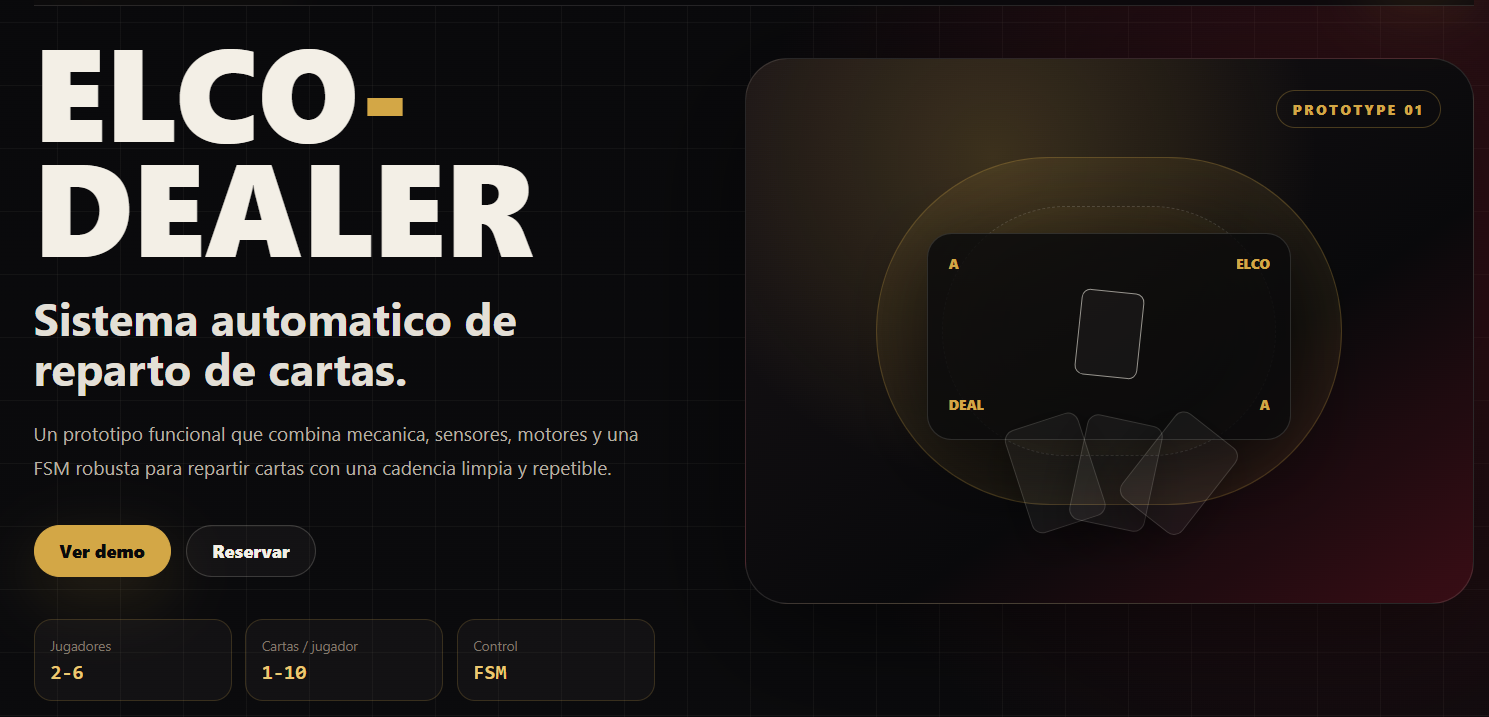
\includegraphics[width=0.85\textwidth]{inicio web (1).png}
    \caption{Interfaz principal de la web ELCO-Dealer con acceso a la Demo y reserva del prototipo.}
    \label{fig:web_hero}
\end{figure}

\subsection{Arquitectura y Contenidos de la Plataforma}

La interfaz ha sido diseñada para segmentar la información en bloques estratégicos, facilitando la comprensión del producto tanto a nivel funcional como técnico:

\begin{itemize}
    \item \textbf{Highlights y Demo:} Esta sección presenta la propuesta de valor del \textbf{ELCO-Dealer}. Incluye un video demostrativo alojado en YouTube que documenta el funcionamiento real del prototipo, su capacidad de barajado automático y el modo de uso para el cliente final (ver Figura \ref{fig:web_hero}).
    
    \item \textbf{Simulador de Reparto:} Herramienta interactiva (Figura \ref{fig:web_simulator}) que permite al usuario visualizar de forma lógica el proceso de distribución de naipes. Este simulador emula el comportamiento del software embebido en la Arduino Mega 2560, manteniendo los límites reales del prototipo (máximo 6 jugadores).
    
    \item \textbf{Engineering (Arquitectura de Software):} Se detalla el diseño orientado a la robustez (Figura \ref{fig:web_arquitectura}), destacando el uso de una \textbf{Máquina de Estados Finitos (FSM)} para gestionar la lógica de control. La web explica cómo el sistema evita bloqueos mediante la implementación de prioridades de eventos, \textit{timeouts} y transiciones claras sin acceso directo a pines para asegurar la portabilidad del código. 
    
    \item \textbf{Hardware y Sensórica:} Bloque técnico que describe la integración de los componentes clave detallados en el listado de materiales (BOM). Se resalta el uso de los drivers \textbf{L298N} para el control de potencia \cite{l298n_st}, el sensor de efecto Hall \textbf{A3144} para la autocalibración de 0 grados y los sensores infrarrojos \textbf{TCRT5000} para la detección de cartas por flancos.
    
    \item \textbf{User Interface (UI):} Detalla el subsistema de configuración. El usuario puede definir interactivamente el número de jugadores y el modo de reparto a través de la pantalla y botonera integradas.
\end{itemize}

\begin{figure}[H]
    \centering
    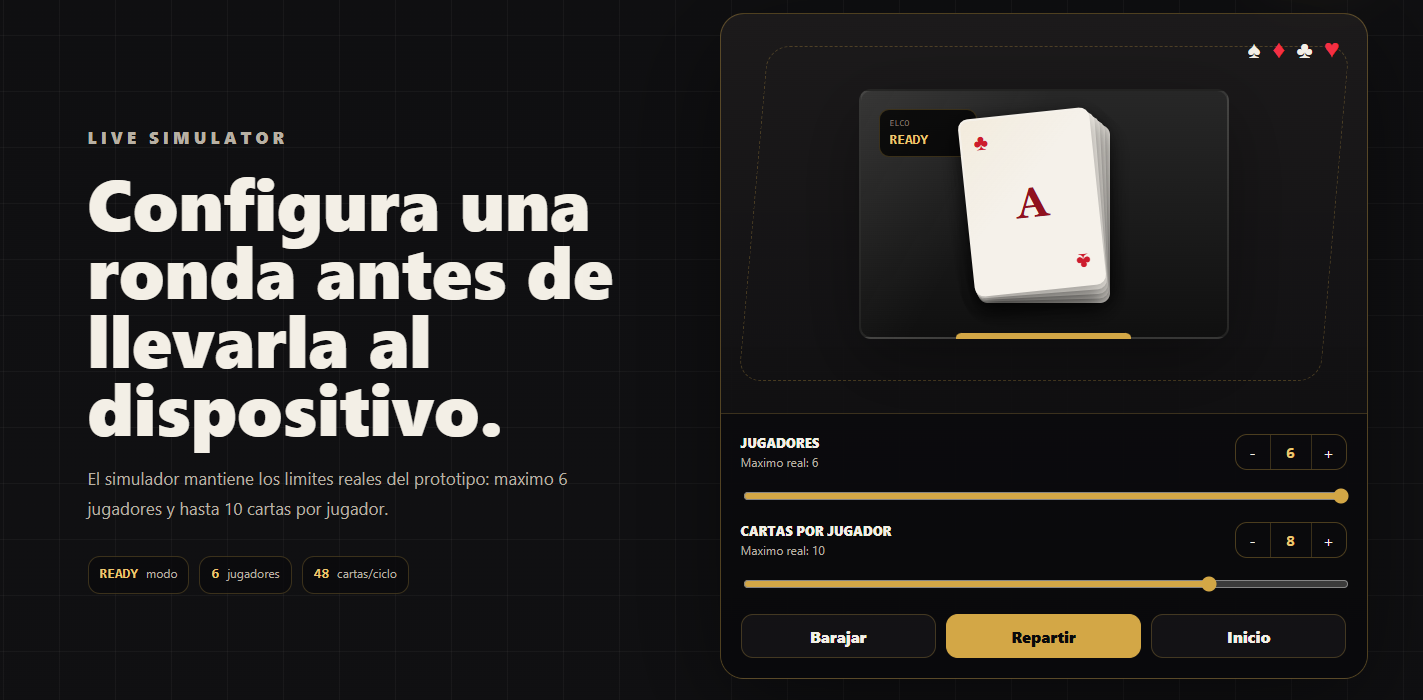
\includegraphics[width=0.85\textwidth]{web simulador.png}
    \caption{Detalle del simulador lógico de barajado y reparto integrado en la plataforma.}
    \label{fig:web_simulator}
\end{figure}

\begin{figure}[H]
    \centering
    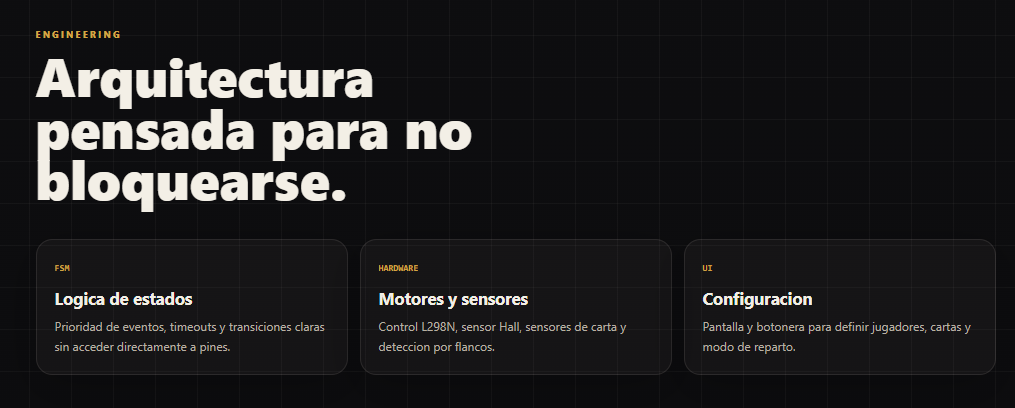
\includegraphics[width=0.85\textwidth]{web arquitectura.png}
    \caption{Detalle de la FSM, el hardware y la UI del prototipo.}
    \label{fig:web_arquitectura}
\end{figure}

\subsection{Estrategia de Captación: Wishlist y Reserva}

Siguiendo un enfoque honesto de lanzamiento de producto bajo el contexto de un proyecto de ingeniería universitaria, la web incluye una sección de reserva (Figura \ref{fig:web_wishlist}). Esta funcionalidad permite registrar el interés de posibles clientes y construir un \textit{storytelling} creíble alrededor del prototipo, alineándose con la viabilidad económica planteada en la memoria del proyecto.

\begin{figure}[H]
    \centering
    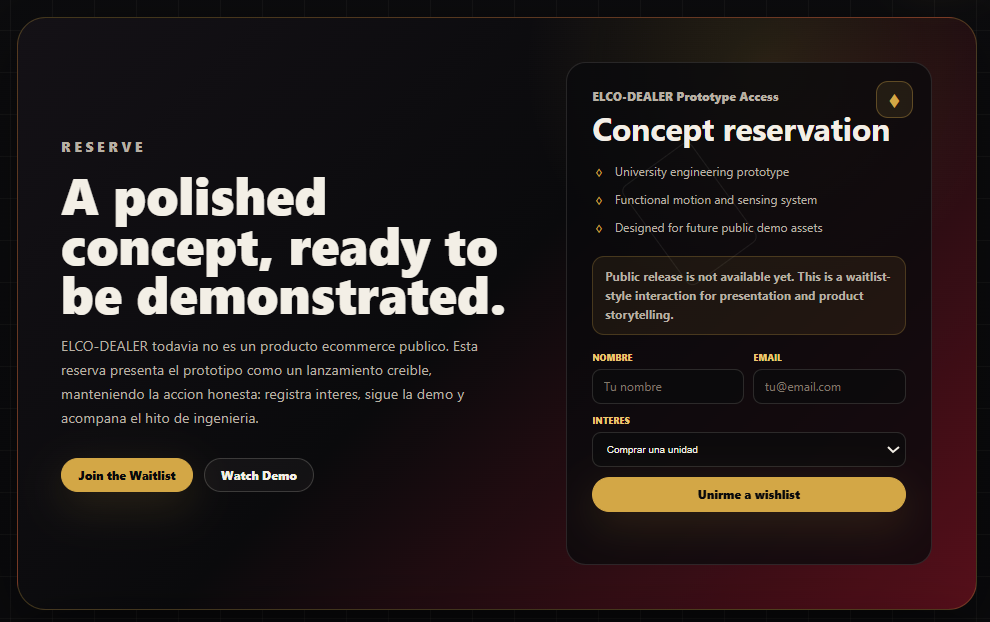
\includegraphics[width=0.85\textwidth]{wishlist.png}
    \caption{Formulario de reserva y wishlist integrado en la plataforma web.}
    \label{fig:web_wishlist}
\end{figure}


\subsection{Integración con la Filosofía Open Source}

En cumplimiento con los requisitos de documentación pública de la asignatura, el pie de página de todas las secciones incluye enlaces directos a los resultados publicados en redes de distribución técnica:
\begin{itemize}
    \item \textbf{GitHub:} Repositorio con el código fuente completo y pruebas de módulos \cite{github_link}.
    \item \textbf{Instructables:} Guía paso a paso para la replicación del proyecto por parte de la comunidad \cite{instructables_link}.
\end{itemize}












\newpage
\section{Conclusión}
El software del \textbf{ELCO-Dealer} se ha planteado como una base robusta para un prototipo físico sometido a tolerancias mecánicas, posibles rebotes de sensores y pequeñas variaciones en el movimiento de cartas. La combinación de una máquina de estados finitos, una capa de hardware centralizada, eventos de usuario priorizados y un modo de diagnóstico permite que el sistema sea comprensible, verificable y ampliable.

Como líneas de mejora software se propone ampliar la capa de sensórica a varios puntos de detección de carta, registrar métricas de fallo durante el uso real, añadir perfiles de calibración por tipo de baraja y conectar la electrónica con la plataforma web o una aplicación móvil en futuras versiones del producto.

\nocite{*}

\newpage
\begingroup
\sloppy
\bibliographystyle{IEEEtran}
\bibliography{refs}
\endgroup


\end{document}
